\section{Paweł Adamczyk}
\label{sec:adpawel}

Aby przejść do kolejnych niezbędnych kroków zastosujemy jeden z trywialnych wzorów rekurencyjnych w całce z funkcji trygonometrycznych:\\ 
$\int\sin^n(ax)dx = -\frac{sin^{n-1}(ax)cos(ax)}{na}+\frac{n-1}{n}\int\sin^{n-2}(ax)dx$

\begin{figure}[htbp]
  \centering
  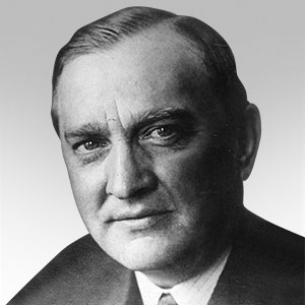
\includegraphics[width=0.7\linewidth]{pictures/banach.jpg}
  \caption{Polski matematyk Stefan Banach}
  \label{fig:banach}
\end{figure}

Wiedza matematyczna pozwala człowiekowi dokonać wielu sukcesów dnia codziennego. Dzięki niej możemy m.in. poprawnie oszacować ilość jabłek, które należy kupić, aby upiec \underline{szarlotkę}, której \href{https://uczymyjakslodzic.pl/szarlotka-prosty-przepis-na-deser-idealny/#Prosta_szarlotka_na_kruchym_ciescie_-_nasz_sprawdzony_przepis}{przepis} umieszczony został poniżej. Jeśli chcesz natomiast poznać kraje, które produkują najwięcej jabłek zobaczysz je w rankingu~\ref{tab:jablka}.\\
\emph{Składniki na ciasto:}
\begin{itemize}
    \item Mąka pszenna – 2 szklanki – 300 g;
    \item Cukier spożywczy – 3 łyżki – 35 g;
    \item Cukier waniliowy – 2 łyżeczki – 10g;
    \item Masło (zimne – prosto z lodówki) – 1 duża kostka – 250 g;
    \item Jajo kurze (zimne – prosto z lodówki) – 1 sztuka;
    \item Proszek do pieczenia lub soda oczyszczona – 2 łyżeczki – 10 g.
\end{itemize}
\emph{Składniki na mus jabłkowy:}
\begin{itemize}
    \item[*] Jabłka (3,00 zł/kg) – 8 – 10 średnich sztuk – ok. 1,8 kg;
    \item[>] Cynamon (6 zł/100g) – 1 łyżeczka – 4 g;
    \item[?] Cukier spożywczy (5,50 zł/kg) – 2 – 3 łyżki – 20 – 35 g.
\end{itemize}

\emph{Sposób przygotowania:}
\begin{enumerate}
    \item Przygotuj ciasto: do miski przesiej mąkę, dodaj cukier spożywczy i waniliowy, a także jajka i proszek do pieczenia. Wymieszaj całość.
    \item Posiekaj zimne masło, dodaj je do zawartości miski i wymieszaj. Następnie wyrabiaj ciasto, aż utworzy spójną, jednolitą konsystencję.
    \item Ciasto owiń w folię spożywczą lub woskowijkę\footnote{woskowijka - kawałek bawełny nasączony woskiem pszczelim, olejem jojoba i żywicą drzewną} i włóż do lodówki.
    \item Przygotuj mus jabłkowy: jabłka umyj, obierz ze skórki, usuń gniazda nasienne i drobno pokrój w kostkę.
    \item Do jabłek dodaj cukier i smaż je w rondelku, aż puszczą odrobinę wody. Jeśli okaże się, że masa jest zbyt wodnista, pogotuj ją trochę dłużej, odparowując nadmiar wody.
    \item Do jabłek dodaj cynamon i odstaw do przestygnięcia.
    \item Piekarnik nagrzej do tem. 180 – 200 st. C.
    \item Formę wyłóż papierem do pieczenia i wyjmij ciasto z lodówki. Podziel je na dwie równe części. Jedną część schowaj do zamrażalnika, a drugą połową wyklejaj spód formy.
    \item Gdy cały spód będzie już gotowy, przełóż masę jabłkową i równomiernie ją rozsmaruj.
    \item Wyjmij z zamrażalnika pozostałą część ciasta i zetrzyj ją na tarce bezpośrednio na jabłka.
    \item Tak przygotowane ciasto wstaw do piekarnika i piecz przez około 60 minut metodą grzanie góra – dół.
    \item Wypieczone ciasto odstaw do ostygnięcia, a następnie podaj z ulubionymi dodatkami.
\end{enumerate}
\vspace{1cm}
\textbf{Matematyka} pomaga w rozumieniu i rozwiązywaniu różnorodnych problemów oraz trudnych sytuacji, z którymi spotykasz się na co dzień. Ucząc się tej dziedziny, zyskujesz umiejętności potrzebne do zarządzania finansami, planowania podróży, gotowania czy wykonywania zadań w pracy. Dzięki \textit{matematyce} możesz podejmować świadome i logiczne decyzje, co wpływa na poprawę jakości Twojego życia.\par
Warto też wspomnieć, że na obliczeniach opiera się informatyka i zawody przyszłości, które są doskonałą trampoliną do wyższych zarobków i zdobycia satysfakcjonującej pracy. Dlatego warto pamiętać o słynnych matematykach takich jak Stefan Banach~\ref{fig:banach}.
\begin{table}[htbp]
\centering
\begin{tabular}{|l|l|l|}
\hline
Miejsce & Kraj/Region       & Produkcja jabłek (w tonach) \\ \hline
1.      & Chiny             & 41 390 000                  \\ \hline
2.      & Stany Zjednoczone & 5 173 670                   \\ \hline
3.      & Turcja            & 3 032 164                   \\ \hline
4.      & Polska            & 2 441 393                   \\ \hline
5.      & Indie             & 2 265 000                   \\ \hline
6.      & Iran              & 2 096 749                   \\ \hline
7.      & Włochy            & 1 921 272                   \\ \hline
8.      & Chile             & 1 766 210                   \\ \hline
9.      & Francja           & 1 710 755                   \\ \hline
10.     & Rosja             & 1 639 421                   \\ \hline
\end{tabular}
\label{tab:jablka}
\caption{Lista krajów największych producentów jabłek}
\end{table}

